\documentclass[10pt]{article}
\usepackage{amsmath}
\usepackage{mathtools}
\DeclarePairedDelimiter{\abs}{\lvert}{\rvert}
\usepackage[hidelinks]{hyperref}
\usepackage{amssymb}
\usepackage{tikz}
\usepackage{caption}
\usepackage{graphicx}
\usepackage[T1]{fontenc}
\graphicspath{{.}}
\usepackage{listings}
\usepackage{verbatim}
\usepackage{floatrow}
\usepackage{bigints}
\lstset{
language=[LaTeX]TeX,
backgroundcolor=\color{gray!25},
basicstyle=\ttfamily,
columns=flexible,
breaklines=true
}
\captionsetup{labelsep=space,justification=centering,singlelinecheck=off}
\reversemarginpar
\usepackage[paper=a4paper,
            %includefoot, % Uncomment to put page number above margin
            marginparwidth=10mm,      % Length of section titles
            marginparsep=0.8mm,       % Space between titles and text
            margin=11mm,              % 25mm margins
            includemp]{geometry}

\begin{document}
\section*{}
\begin{flushleft}
Name: Krishna Chaitanya Sripada\\
\end{flushleft}
\section*{Ans 1}
\begin{flushleft}
The generated samples are:\\
\begin{lstlisting}
1 [[-0.97977299]
 [ 0.00842229]
 [-0.81230254]
 ..., 
 [-0.02064795]
 [-0.514107  ]
 [ 0.5813556 ]]
2 [[ 0.125146   -0.40207117]
 [-0.82553458  0.08322131]
 [-0.93928138  0.08880301]
 ..., 
 [ 0.26225264 -0.85643974]
 [-0.0297685  -0.66172214]
 [ 0.2369696   0.73281328]]
3 [[ 0.1545676  -0.88476312  0.37538976]
 [-0.076204    0.77983112 -0.24302431]
 [-0.79693234 -0.19104474  0.08678971]
 ..., 
 [ 0.46406434 -0.70798911 -0.42797605]
 [-0.0982297  -0.17806004  0.92219372]
 [-0.12246412  0.52546831  0.12582817]]
4 [[-0.10995823 -0.09060495  0.18391883 -0.25517966]
 [-0.44176387  0.00365563 -0.00300895 -0.66249913]
 [ 0.31395478 -0.28075808  0.07659535  0.57308922]
 ..., 
 [-0.40635851 -0.69734769  0.05903802 -0.39497366]
 [-0.61739903 -0.44575521  0.10770923  0.06502449]
 [ 0.35055945  0.09720481  0.75759123 -0.47176295]]
 \end{lstlisting}
I've just displayed the first 4 samples to show the generation of 10000 samples using the algorithm 1. Note that this is not the complete set of samples generated ( as seen by the ellipsis in the output).
\end{flushleft}
\section*{Ans 2}
\begin{flushleft}
\begin{figure}[!htb]
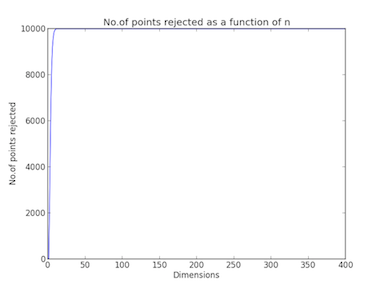
\includegraphics{2.png}
\caption{:No.of points rejected as a function of `n'}
\end{figure}
As we can see from the above figure, for dimensions 1 to 13, the points rejected are 0, 2106, 4734, 6924, 8386, 9202, 9615, 9836, 9933, 9975, 9993, 9999, 9998 and from dimensions 14 to 400, we see that all the points are rejected i.e., all points are inside the cube $[-1, 1]^{n}$ but not inside the ball $B^{n}(1)$.
\end{flushleft}
\vspace{10em}
\section*{Ans 3}
\begin{flushleft}
The generated samples are:\\
\begin{lstlisting}
2 [[[-0.65692011  1.16783918]]

 [[ 0.82797408 -1.39857805]]

 [[ 0.1461279   0.13553733]]

 ..., 
 [[-0.04946436  1.12446543]]

 [[ 0.91540538 -0.21908985]]

 [[ 0.81293634 -2.28027548]]]
5 [[[-1.2456768   1.80039919  1.17679543 -0.69789122 -0.76721011]]

 [[-2.08692172  0.51378863  2.156899    0.4165659  -0.4891643 ]]

 [[ 0.00469149  1.79521765  0.23825432 -0.1498503  -0.46991127]]

 ..., 
 [[-0.72383131 -1.01382281 -0.30672538  0.68511039  0.17310003]]

 [[-0.27179642 -0.82979279  0.16814383  0.76172546 -0.53268273]]

 [[-1.19568478 -1.71578359 -0.35880254  0.32901967  0.41580998]]]
10 [[[-2.11815605 -0.35731693  1.6130568  ...,  1.25442419  1.56232948
    0.35447931]]

 [[-0.13652401  1.37226018 -0.76691262 ..., -0.95764159  0.09348221
   -1.41324988]]

 [[-1.41626515  0.42959637 -0.72194693 ...,  0.16525344 -1.43592195
   -0.41799285]]

 ..., 
 [[-0.97485073  0.44934148 -0.38081946 ..., -0.07637263  1.10600349
    0.61022057]]

 [[ 0.24000133 -0.71633007  0.41135705 ..., -1.20362708 -0.6297904
    0.05049542]]

 [[-2.56336523  1.33890549  0.52369033 ..., -0.73657761  1.36940211
    1.38825666]]]
15 [[[-0.80481799  1.81004443 -0.02678096 ..., -0.3047872   0.57138172
   -0.23113882]]

 [[-0.13910619  1.08208882 -0.72344492 ...,  0.56388572 -1.4720767
    0.2459732 ]]

 [[-1.40338075 -0.48069908  0.01378676 ..., -0.44783218 -2.6447068
   -0.01177376]]

 ..., 
 [[-1.62982492 -0.22021754  0.60822971 ..., -0.0808899   1.64250104
    0.78917796]]

 [[-0.25659009 -0.1753043  -1.20571977 ..., -1.35860634  1.46238483
   -0.31844546]]

 [[-1.0764558   0.27053731  0.16825497 ..., -0.78778908  0.64355262
   -1.47627777]]]
20 [[[ 0.29053213 -0.98661741 -1.12983281 ..., -1.02831458  0.31240548
   -0.21604852]]

 [[-0.03431936 -0.2834155  -0.19163956 ..., -0.91225312 -0.19950807
   -0.58912561]]

 [[-1.4425197   0.13178094  0.95207496 ..., -0.64722797  1.27522824
    1.29144633]]

 ..., 
 [[-1.42532757 -0.20938423 -0.67902917 ..., -0.48856252 -1.38059591
   -0.00405272]]

 [[-0.91422073 -0.33843193  1.19571491 ..., -0.48680666 -0.64461441
    0.87500838]]

 [[ 0.49749863  0.82310547 -0.95117333 ...,  0.09735673  0.79174279
   -1.3268248 ]]]
 \end{lstlisting}
 I've used a numpy array and because of that, not all the samples are displaced in the output. ( as seen by the ellipsis in the output).
\end{flushleft}
\section*{Ans 4}
\begin{flushleft}
\begin{figure}[!htb]
    \begin{floatrow}
         \ffigbox{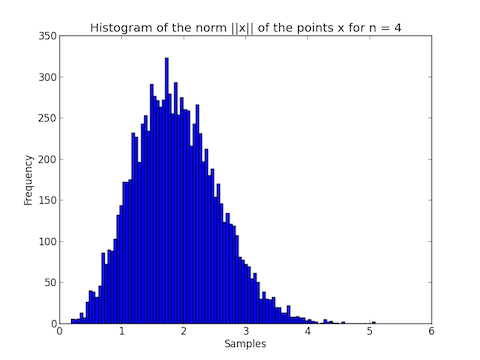
\includegraphics[scale = 0.8]{4_hist.png}}{\caption{:Histogram for n =4}\label{:Histogram for n =4}}
         \ffigbox{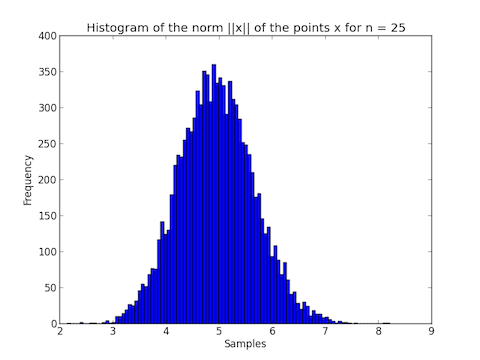
\includegraphics[scale = 0.8]{25_hist.png}}{\caption{:Histogram for n =25}\label{25}}
    \end{floatrow}
\end{figure}
\begin{figure}[!htb]
    \begin{floatrow}
         \ffigbox{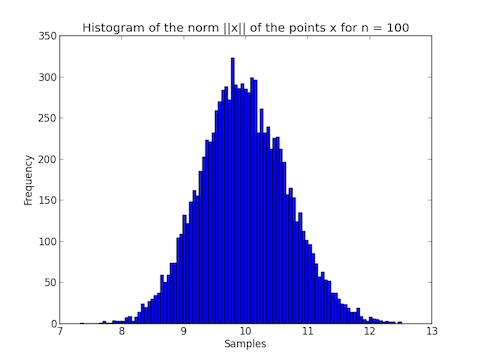
\includegraphics[scale = 0.8]{100_hist.png}}{\caption{:Histogram for n =100}\label{100}}
         \ffigbox{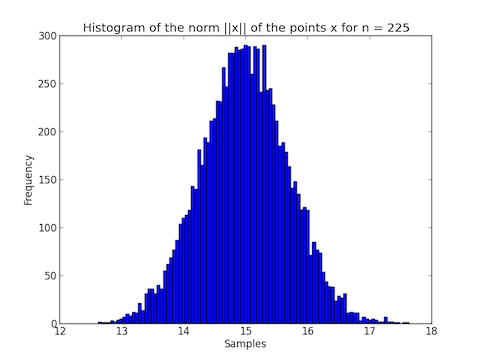
\includegraphics[scale = 0.8]{225_hist.png}}{\caption{:Histogram for n =225}\label{225}}
    \end{floatrow}
\end{figure}
\begin{figure}[!htb]
    \begin{floatrow}
          \ffigbox{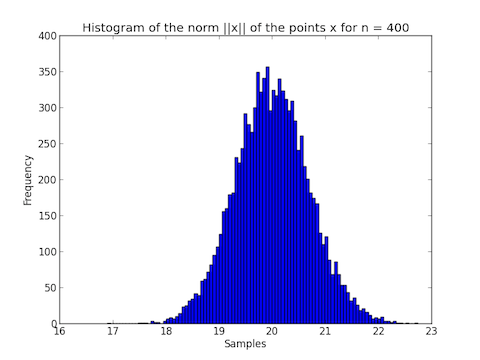
\includegraphics[scale = 0.8]{400_hist.png}}{\caption{:Histogram for n =400}\label{400}}
    \end{floatrow}
\end{figure}
\end{flushleft}
\vspace{20em}
\section*{Ans 5}
\begin{flushleft}
\begin{figure}[!htb]
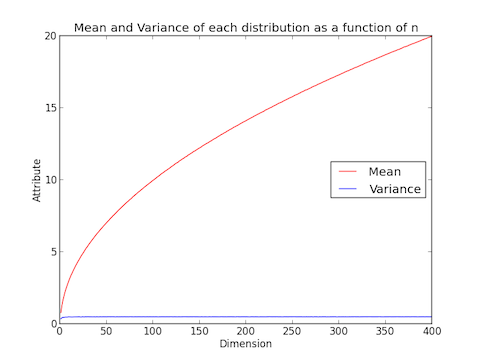
\includegraphics[scale = 0.8]{6.png}
\caption{:Mean and Variance as a function of `n'}
\end{figure}
We notice that the variance values don't change as the dimension increases. The mean varies as $\sqrt{n}$ as the dimension increases.
\end{flushleft}
\section*{Ans 6}
\begin{flushleft}
Given that,\\
$\gamma(A) = \frac{1}{(2\pi)^\frac{n}{2}} \bigintss_{A} e^{-\frac{\parallel x \parallel^{2}}{2}} dx$\\
Therefore,\\
$\gamma(x \in \mathbb{R} ^{n}: f(x) \leq a) = \frac{1}{(2\pi)^\frac{n}{2}} \bigintss_{x: f(x) \leq a} e^{-\frac{\parallel x \parallel^{2}}{2}} dx$\\
Expanding this, we get,\\
$\gamma(x \in \mathbb{R} ^{n}: f(x) \leq a) \leq \frac{1}{(2\pi)^\frac{n}{2}} \bigintss_{x: f(x) \leq a} e^{-\frac{\sum_{i=1}^{n} x_{i}^{2}}{2}} dx_{1} \ldots dx_{n}$\\
\vspace{0.5em}
Also given that,\\
$d\gamma(x) = \frac{1}{(2\pi)^\frac{n}{2}} e^{-\frac{\sum_{i=1}^{n} x_{i}^{2}}{2}} dx_{1} \ldots dx_{n}$\\
\vspace{0.5em}
Using the above equation, we get,\\
$\gamma(x \in \mathbb{R} ^{n}: f(x) \leq a) \leq \frac{1}{(2\pi)^\frac{n}{2}} \bigintss_{x: f(x) \leq a} (2\pi)^\frac{n}{2} d \gamma(x)$\\
\vspace{0.5em}
$\gamma(x \in \mathbb{R} ^{n}: f(x) \leq a) \leq \bigintss_{x: f(x) \leq a} d \gamma(x)$\\
Multiplying $e^{-\lambda a}$, on both sides, we get,\\
\vspace{0.5em}
$e^{-\lambda a} \gamma(x \in \mathbb{R} ^{n}: f(x) \leq a) \leq e^{-\lambda a} \bigintss_{x: f(x) \leq a} d \gamma(x)$\\
\vspace{0.5em}
$e^{-\lambda a} \gamma(x \in \mathbb{R} ^{n}: f(x) \leq a) \leq \bigintss_{x: f(x) \leq a} e^{-\lambda f(x)} d \gamma(x)$\\
\vspace{0.5em}
$\gamma(x \in \mathbb{R} ^{n}: f(x) \leq a) \leq e^{\lambda a} \bigintss_{x: f(x) \leq a} e^{-\lambda f(x)} d \gamma(x)$\\
\vspace{0.5em}
Since $f: \mathbb{R} ^{n} \rightarrow \mathbb{R}$,\\
\vspace{0.5em}
$\gamma\{x \in \mathbb{R} ^{n}: f(x) \leq a\} \leq e^{\lambda a} \bigintss_{\mathbb{R} ^{n}}^{\mathbb{R}} e^{-\lambda f(x)} d \gamma(x)$\\
\end{flushleft}
\section*{Ans 7}
\begin{flushleft}
Replacing $f(x) = \frac{\parallel x \parallel ^{2}}{2}$ and using $a = \frac{(n - \delta)}{2}$, we get,\\
\vspace{0.5em}
$\gamma(x \in \mathbb{R} ^{n}: \frac{\parallel x \parallel ^{2}}{2} \leq \frac{(n - \delta)}{2}) \leq e^{\frac{\lambda (n - \delta)}{2}} \bigintss_{\mathbb{R} ^{n}}^{\mathbb{R}} e^{\frac{-\lambda \parallel x \parallel ^{2}}{2}} d \gamma(x)$\\
\vspace{0.5em}
From the equations given in the question, we get,\\
\vspace{0.5em}
$d \gamma(x) = \frac{1}{(2\pi)^\frac{n}{2}} e^{-\frac{\parallel x \parallel^{2}}{2}} dx$\\
Upon replacement, we get,\\
\vspace{0.5em}
$\gamma(x \in \mathbb{R} ^{n}: \frac{\parallel x \parallel ^{2}}{2} \leq \frac{(n - \delta)}{2}) \leq e^{\frac{\lambda (n - \delta)}{2}} \bigintss_{\mathbb{R} ^{n}}^{\mathbb{R}} e^{\frac{-\lambda \parallel x \parallel ^{2}}{2}} \frac{1}{(2\pi)^\frac{n}{2}} e^{-\frac{\parallel x \parallel^{2}}{2}} dx$\\
This simplifies to,\\
\vspace{0.5em}
$\gamma\{x \in \mathbb{R} ^{n}: \parallel x \parallel ^{2} \leq (n - \delta)\} \leq e^{\frac{\lambda (n - \delta)}{2}} \frac{1}{(2\pi)^\frac{n}{2}}  \bigintss_{\mathbb{R} ^{n}}^{\mathbb{R}} e^{\frac{-(\lambda +1)\parallel x \parallel ^{2}}{2}} dx$\\
\end{flushleft}
\section*{Ans 8}
\begin{flushleft}
Given that $ y = x\sqrt{1+\lambda}$ and \\
\vspace{0.5em}
$\frac{1}{(2\pi)^\frac{n}{2}}  \bigintss_{\mathbb{R} ^{n}} e^{\frac{-(\lambda +1)\parallel x \parallel ^{2}}{2}} dx = \frac{1}{(1+\lambda)^{\frac{n}{2}}}$\\
\vspace{0.5em}
If $\lambda = \frac{\delta}{(n - \delta)}$, we get, \\
\vspace{0.5em}
$\gamma\{x \in \mathbb{R} ^{n}: \parallel x \parallel ^{2} \leq (n - \delta)\} \leq e^{\frac{\frac{\delta}{(n - \delta)} (n - \delta)}{2}} \frac{1}{(1+\lambda)^{\frac{n}{2}}}$\\
\vspace{0.5em}
$\gamma\{x \in \mathbb{R} ^{n}: \parallel x \parallel ^{2} \leq (n - \delta)\} \leq e^{\frac{\delta}{2}} \frac{1}{(1+\frac{\delta}{(n - \delta)})^{\frac{n}{2}}}$\\
Upon simplification, we get,\\
\vspace{0.5em}
$\gamma\{x \in \mathbb{R} ^{n}: \parallel x \parallel ^{2} \leq (n - \delta)\} \leq e^{\frac{\delta}{2}} (\frac{n- \delta}{n}) ^ {\frac{n}{2}}$\\
\end{flushleft}
\section*{Ans 9}
\begin{flushleft}
If $\epsilon = \frac{\delta}{n}$ and since $\ln(1-x) + x \leq \frac{-x^{2}}{2}$, we get,\\
\vspace{0.5em}
$\gamma\{x \in \mathbb{R} ^{n}: \parallel x \parallel ^{2} \leq (n - n \epsilon)\} \leq e^{\frac{n \epsilon}{2}} (\frac{n- n \epsilon}{n}) ^ {\frac{n}{2}}$\\
\vspace{0.5em}
$\gamma\{x \in \mathbb{R} ^{n}: \parallel x \parallel ^{2} \leq n(1 - \epsilon)\} \leq e^{\frac{n \epsilon}{2}} (1 - \epsilon) ^ {\frac{n}{2}}$\\
Taking $\ln$ on both sides, we get,\\
\vspace{0.5em}
$\ln (\gamma\{x \in \mathbb{R} ^{n}: \parallel x \parallel ^{2} \leq n(1 - \epsilon)\}) \leq \frac{n \epsilon}{2} + \frac{n}{2} \ln(1 - \epsilon)$\\
\vspace{0.5em}
$\ln (\gamma\{x \in \mathbb{R} ^{n}: \parallel x \parallel ^{2} \leq n(1 - \epsilon)\}) \leq \frac{n}{2} (\ln(1 - \epsilon) + \epsilon)$\\
Upon simplification, we get,\\
\vspace{0.5em}
$\ln (\gamma\{x \in \mathbb{R} ^{n}: \parallel x \parallel ^{2} \leq n(1 - \epsilon)\}) \leq - \frac{n}{2} (\frac{\epsilon^{2}}{2})$\\
\vspace{0.5em}
$\gamma\{x \in \mathbb{R} ^{n}: \parallel x \parallel ^{2} \leq n(1 - \epsilon)\} \leq e^{-\frac{n \epsilon^{2}}{4}}$\\
\end{flushleft}
\vspace{10em}
\section*{Ans 10}
\begin{flushleft}
Given, \\
\vspace{0.5em}
$\gamma\{x \in \mathbb{R} ^{n}: \parallel x \parallel ^{2} \leq n(1 - \epsilon)\} \leq e^{-\frac{n \epsilon^{2}}{4}}$\\
and, \\
\vspace{0.5em}
$\gamma\{x \in \mathbb{R} ^{n}: \parallel x \parallel ^{2} \geq n(1 + \epsilon)\} \leq e^{-\frac{n \epsilon^{2}}{8}}$\\
\vspace{0.5em}
Combining the above two equations and taking $\ln$ on both sides, we get,\\
\vspace{0.5em}
$\ln(\gamma\{x \in \mathbb{R} ^{n}: \parallel x \parallel ^{2} \leq n(1 - \epsilon)\}) \leq -\frac{n \epsilon^{2}}{4}$\\
\vspace{0.5em}
$\ln(\gamma\{x \in \mathbb{R} ^{n}: \parallel x \parallel ^{2} \geq n(1 + \epsilon)\}) \leq -\frac{n \epsilon^{2}}{8}$\\
\vspace{0.5em}
Subtracting above two equations, we get, \\
\vspace{0.5em}
$\ln(\gamma\{x \in \mathbb{R} ^{n}: \parallel x \parallel ^{2} \leq n(1 - \epsilon)\}) - \ln(\gamma\{x \in \mathbb{R} ^{n}: \parallel x \parallel ^{2} \geq n(1 + \epsilon)\}) \leq -\frac{n \epsilon^{2}}{8}$\\
\vspace{0.5em}
$\ln(\frac{\gamma\{x \in \mathbb{R} ^{n}: \parallel x \parallel ^{2} \leq n(1 - \epsilon)\}}{\gamma\{x \in \mathbb{R} ^{n}: \parallel x \parallel ^{2} \geq n(1 + \epsilon)\}}) \leq -\frac{n \epsilon^{2}}{8}$\\
\vspace{0.5em}
$\frac{\gamma\{x \in \mathbb{R} ^{n}: \parallel x \parallel ^{2} \leq n(1 - \epsilon)\}}{\gamma\{x \in \mathbb{R} ^{n}: \parallel x \parallel ^{2} \geq n(1 + \epsilon)\}} \leq e^{-\frac{n \epsilon^{2}}{8}}$\\
\vspace{0.5em}
$\frac{\gamma\{x \in \mathbb{R} ^{n}: \parallel x \parallel ^{2} - n + n \epsilon \leq 0 \}}{\gamma\{x \in \mathbb{R} ^{n}: n + n\epsilon -\parallel x \parallel ^{2}  \leq 0 \}} \leq e^{-\frac{n \epsilon^{2}}{8}}$\\
\vspace{0.5em}
Applying dividendo, we get,\\
\vspace{0.5em}
$\gamma\{x \in \mathbb{R} ^{n}: \frac{2(\parallel x \parallel ^{2} - n)}{2 n \epsilon} \leq 0\} \leq \frac{e^{-\frac{n \epsilon^{2}}{8}} -1}{e^{-\frac{n \epsilon^{2}}{8}} +1} \leq e^{-\frac{n \epsilon^{2}}{8}} \leq 2 e^{-\frac{n \epsilon^{2}}{8}}$\\
\vspace{0.5em}
$\gamma\{x \in \mathbb{R} ^{n}:  \left|\frac{\parallel x \parallel ^{2}}{n} -1\right| \geq \epsilon \} \leq 2 e^{-\frac{n \epsilon^{2}}{8}}$\\
\end{flushleft}
\section*{Ans 11}
\begin{flushleft}
We can be that from Eq(11) and Eq(12), we get,\\
$\gamma\{x \in \mathbb{R} ^{n}: \parallel x \parallel \leq \sqrt{n(1 - \epsilon)}\} \leq e^{-\frac{n \epsilon^{2}}{4}}$\\
$\gamma\{x \in \mathbb{R} ^{n}: \parallel x \parallel \geq \sqrt{n(1 + \epsilon)}\} \leq e^{-\frac{n \epsilon^{2}}{8}}$\\
Since the concentration of measure is a little lesser than $\sqrt{n}$ as $\parallel x \parallel \leq \sqrt{n(1 - \epsilon)}$ and little higher than $\sqrt{n}$ as $\parallel x \parallel \geq \sqrt{n(1 + \epsilon)}$, we can say that the Gaussian measure is concentrated on the sphere of radius $\sqrt{n}$ with a decay of $e^{\frac{-\epsilon^{2}}{8}}$.
\end{flushleft}
\section*{Ans 12}
\begin{flushleft}
\begin{figure}[!htb]
    \begin{floatrow}
         \ffigbox{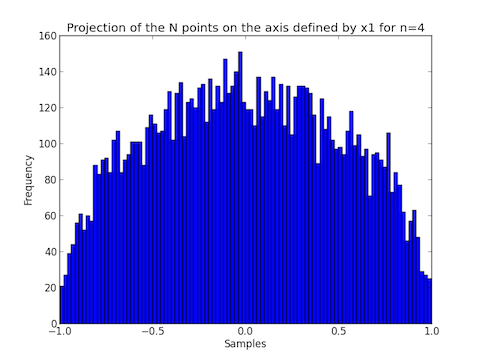
\includegraphics[scale = 0.8]{hist_4.png}}{\caption{:Histogram for n = 4}\label{4}}
         \ffigbox{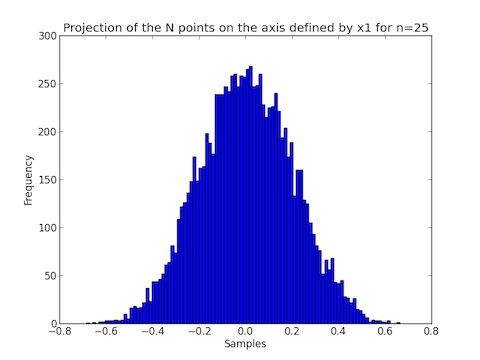
\includegraphics[scale = 0.8]{hist_25.png}}{\caption{:Histogram for n =25}\label{25}}
    \end{floatrow}
\end{figure}
\begin{figure}[!htb]
    \begin{floatrow}
         \ffigbox{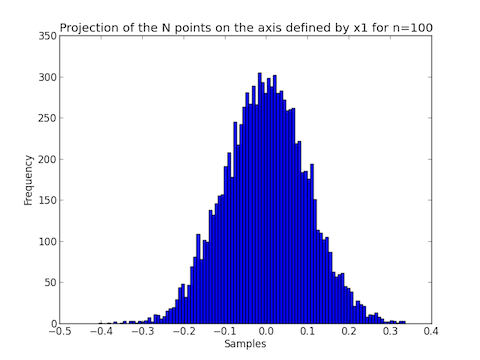
\includegraphics[scale = 0.8]{hist_100.png}}{\caption{:Histogram for n = 100}\label{100}}
         \ffigbox{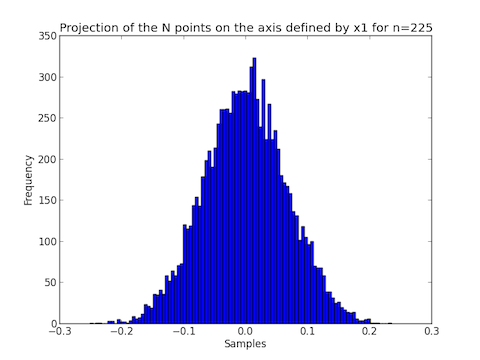
\includegraphics[scale = 0.8]{hist_225.png}}{\caption{:Histogram for n =225}\label{225}}
    \end{floatrow}
\end{figure}
\begin{figure}[!htb]
    \begin{floatrow}
         \ffigbox{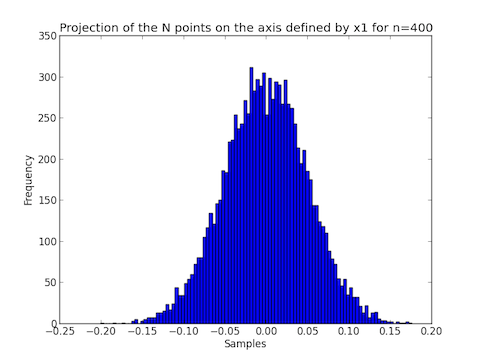
\includegraphics[scale = 0.8]{hist_400.png}}{\caption{:Histogram for n = 400}\label{400}}
    \end{floatrow}
\end{figure}
\end{flushleft}
\vspace{10em}
\section*{Ans 13}
\begin{flushleft}
\begin{figure}[!htb]
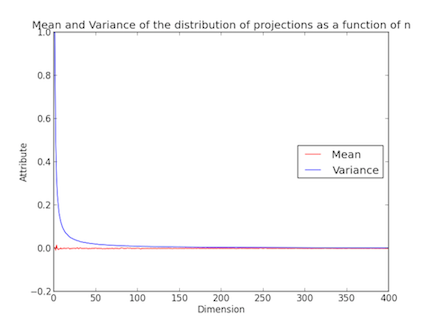
\includegraphics{13.png}
\caption{:Mean and Variance of the distribution of the projections}
\end{figure}
\end{flushleft}
\section*{Ans 14}
\begin{flushleft}
\begin{figure}[!htb]
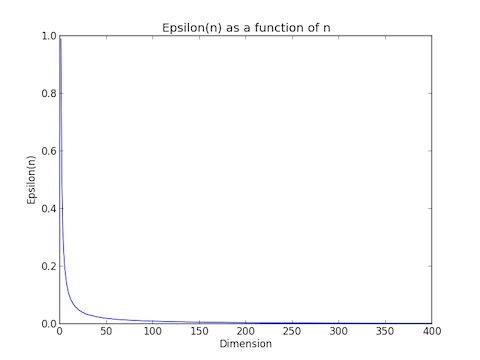
\includegraphics{14_2.png}
\caption{:Plot for $\epsilon(n)$ as a function of n}
\end{figure}
This curve is similar to the exponential decay curve where we can see that as the dimension increases, the value of $\epsilon(n)$ reaches close to 0.
\end{flushleft}
\section*{Ans 15}
\begin{flushleft}
The choice of axis ($x_{1}$ versus any other axis) is not important as the results of projecting the points onto the axis remains the same regardless of the axes chosen. Since the points are randomly chosen, they follow the same distribution and thus we notice the symmetry in the points.\\
\end{flushleft}
\section*{Ans 16}
\begin{flushleft}
\begin{lstlisting}
4 [[ 0.63028936 -1.097736    0.93835393  1.2317479 ]
 [-1.20713363  1.27085457 -0.43553443 -0.85910816]
 [ 1.68404095 -0.30129244  0.37521483 -0.96563077]
 ..., 
 [-0.18374822 -0.61523148  1.8802388  -0.22897355]
 [-0.9860119  -0.75993342  1.2928199   0.88255223]
 [-0.04117349 -0.44859436 -1.35485332 -1.40051431]]
25 [[ 0.68799096 -0.26786441 -0.68556769 ..., -0.07891129  2.22662855
  -0.66184881]
 [ 0.36996842 -1.05560762 -2.35133188 ...,  0.62801174  0.57403549
   1.16396758]
 [-1.0262364   1.72229894 -2.09451358 ..., -0.7085281  -0.6868293
  -0.28082034]
 ..., 
 [-0.61785262  0.76006305  0.48852513 ..., -1.10566109 -0.72852901
  -1.1394798 ]
 [-1.21689115  1.69291832  1.49669937 ..., -0.58510604 -1.11935484
  -1.0218551 ]
 [ 0.46226122  1.32115449  1.36879548 ...,  1.67600523  0.62818761
   0.66409739]]
100 [[-1.41846347 -0.11382888  3.141689   ..., -0.55453294 -0.82674094
  -0.05748162]
 [-0.30089584  0.15039451 -1.38820549 ...,  0.898891    0.15666097
   2.06694431]
 [-0.85606152 -1.24574924  0.85788595 ...,  2.06564677 -2.22904304
   2.13899737]
 ..., 
 [ 1.16194303  0.30843398 -0.06935013 ..., -1.06148569 -0.32450694
  -0.19570746]
 [ 0.47265695 -1.5127091  -0.48501618 ..., -1.12642233  0.11579328
   1.50321864]
 [-0.43713988 -0.20868236  0.36851884 ..., -0.05434654  0.05375461
  -0.15957454]]
225 [[ 0.07051839 -1.05894358 -1.61087903 ..., -0.9888515   1.87658628
   1.5854141 ]
 [ 1.27572116  0.7610539  -1.74757944 ...,  0.01515552 -0.73937378
  -0.03770229]
 [-2.21061224  0.45518723 -0.70741455 ...,  1.66380623  0.78883653
  -0.08602367]
 ..., 
 [ 1.82828175  1.59886912  0.12101186 ...,  0.67458581  0.20624187
   0.75808681]
 [ 0.90236545 -0.39523239 -2.28663612 ...,  0.54438564  2.0427492
  -0.59887064]
 [ 0.33834693 -0.47356384  0.41578749 ..., -0.33740048 -0.93787427
   0.24766759]]
400 [[-1.56539675 -0.16155796  1.5748229  ...,  0.15596077  1.85347936
  -0.02557695]
 [ 0.40660968  2.04050084 -0.90966779 ...,  1.55023846 -0.98069676
   0.21059077]
 [-0.54338601  2.2325388  -2.04107933 ...,  0.39092473 -0.15738214
  -0.05136597]
 ..., 
 [ 1.45327995  0.02588449  0.70836157 ...,  0.63640216  0.06611108
   0.18656551]
 [ 0.01239606 -1.71669257  0.60640558 ...,  0.58437235  0.04035378
  -0.62907416]
 [-0.50045222  0.40013465 -0.64167211 ...,  0.31144153 -2.17281477
  -1.0930534 ]]
\end{lstlisting}
I've used a numpy array and because of that, not all the samples are displaced in the output. ( as seen by the ellipsis in the output).
\end{flushleft}
\section*{Ans 17}
\begin{flushleft}
\begin{figure}[!htb]
    \begin{floatrow}
         \ffigbox{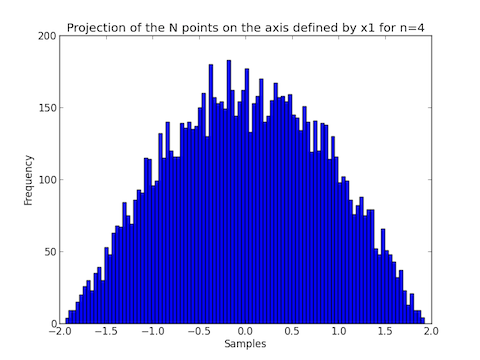
\includegraphics[scale = 0.8]{17_hist_4.png}}{\caption{:Histogram for n = 4}\label{4}}
         \ffigbox{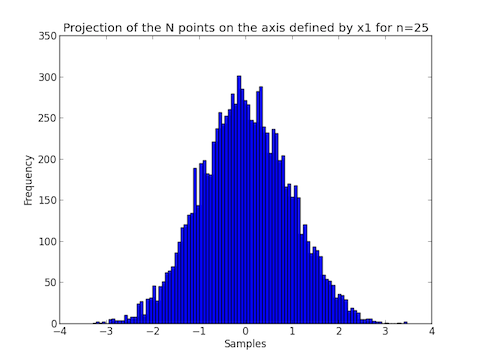
\includegraphics[scale = 0.8]{17_hist_25.png}}{\caption{:Histogram for n =25}\label{25}}
    \end{floatrow}
\end{figure}
\begin{figure}[!htb]
    \begin{floatrow}
         \ffigbox{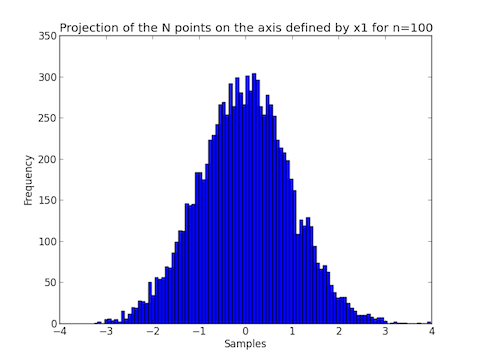
\includegraphics[scale = 0.8]{17_hist_100.png}}{\caption{:Histogram for n = 100}\label{100}}
         \ffigbox{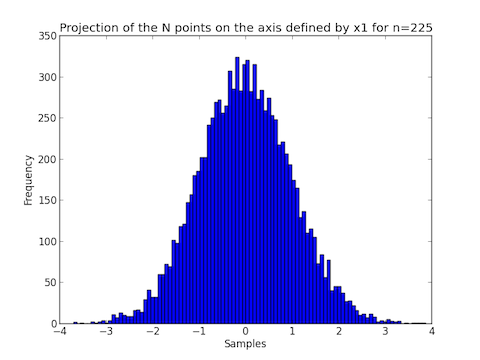
\includegraphics[scale = 0.8]{17_hist_225.png}}{\caption{:Histogram for n =225}\label{225}}
    \end{floatrow}
\end{figure}
\begin{figure}[!htb]
    \begin{floatrow}
         \ffigbox{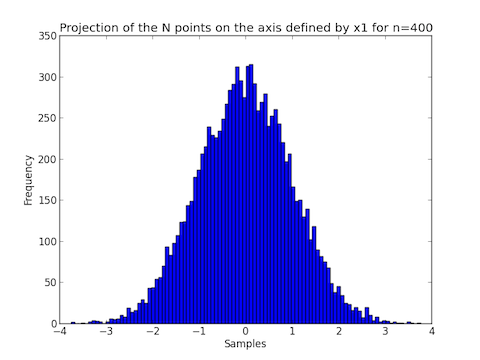
\includegraphics[scale = 0.8]{17_hist_400.png}}{\caption{:Histogram for n = 400}\label{400}}
    \end{floatrow}
\end{figure}
\end{flushleft}
\section*{Ans 18}
\begin{flushleft}
\begin{figure}[!htb]
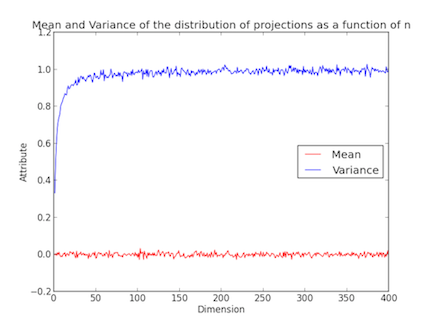
\includegraphics{18.png}
\caption{:Mean and Variance of the distribution of the projections}
\end{figure}
We observe that the mean is always close to 0 regardless of the dimension and the variance reaches 1 after a certain dimension and then remains close to 1 as the dimension keeps increasing.
\end{flushleft}
\section*{Ans 19}
\begin{flushleft}
\begin{figure}[!htb]
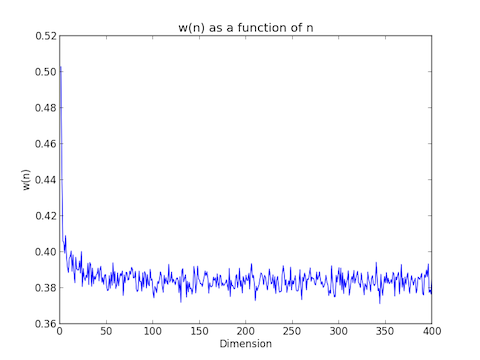
\includegraphics{19.png}
\caption{:Plot w(n) as a function of n}
\end{figure}
We observe an exponential decay curve where the relative volume is high as the dimension is low and once the dimension increases, we see that the volume falls down to a certain value and remains more or less around the same value for higher dimensions.\\
\end{flushleft}
\section*{Ans 20}
\begin{flushleft}
No, the choice of axis ($x_{1}$ versus any other axis) is not important for the results in the previous answer. Since the points are randomly chosen, they follow the same distribution and thus we notice the symmetry in the points.\\
\end{flushleft}
\section*{Ans 21}
\begin{flushleft}
\begin{figure}[!htb]
    \begin{floatrow}
         \ffigbox{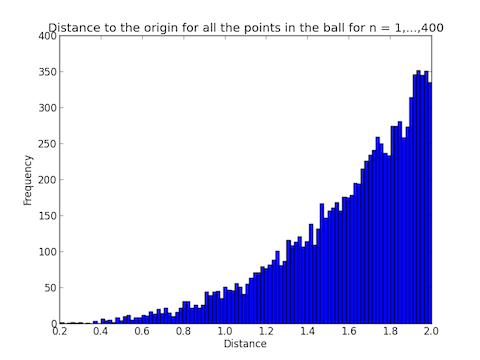
\includegraphics[scale = 0.8]{21_hist_4.png}}{\caption{:Histogram for n = 4}\label{4}}
         \ffigbox{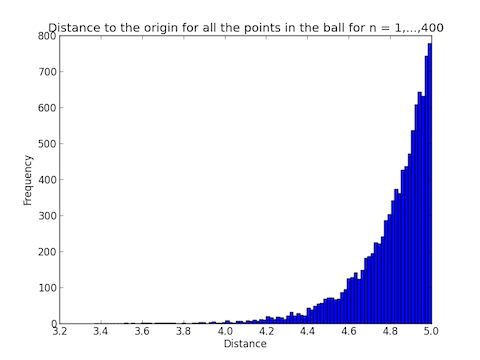
\includegraphics[scale = 0.8]{21_hist_25.png}}{\caption{:Histogram for n =25}\label{25}}
    \end{floatrow}
\end{figure}
\begin{figure}[!htb]
    \begin{floatrow}
         \ffigbox{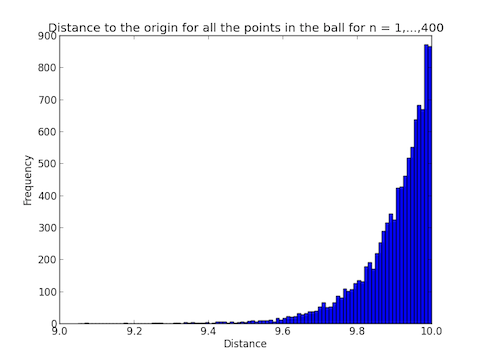
\includegraphics[scale = 0.8]{21_hist_100.png}}{\caption{:Histogram for n = 100}\label{100}}
         \ffigbox{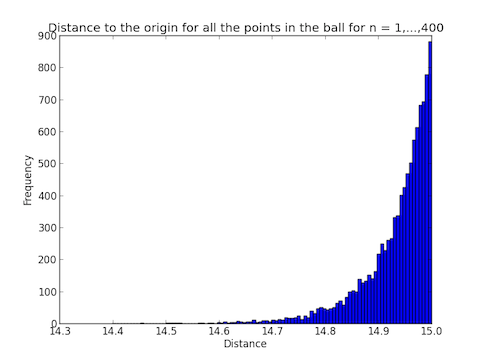
\includegraphics[scale = 0.8]{21_hist_225.png}}{\caption{:Histogram for n =225}\label{225}}
    \end{floatrow}
\end{figure}
\begin{figure}[!htb]
    \begin{floatrow}
         \ffigbox{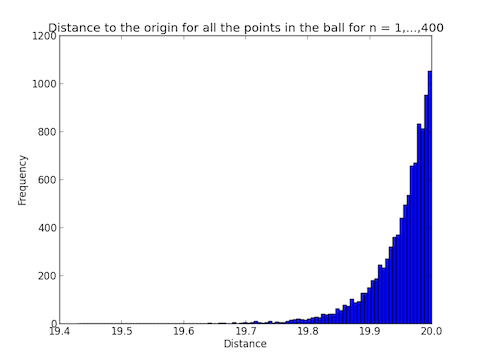
\includegraphics[scale = 0.8]{21_hist_400.png}}{\caption{:Histogram for n = 400}\label{400}}
    \end{floatrow}
\end{figure}
The apparent paradox is that we see that the concentration points reaches its maximum at the radius value = $\sqrt{n}$ unlike the concentration measure which also has the highest concentration at the radius and follows the Gaussian distribution, this doesn't.\\
\end{flushleft}
\section*{Ans 22}
\begin{flushleft}
\lstinputlisting[breaklines]{problem22.py}
\textbf{Result:}\\
\begin{lstlisting}
Wigner Matrix for Bernoulli
[[-1. -1. -1.]
 [-1. -1. -1.]
 [-1. -1.  1.]]
[[-1. -1.  1.  1.]
 [-1. -1. -1. -1.]
 [ 1.  1.  1.  1.]
 [-1. -1.  1.  1.]]
[[ 1.  1.  1. -1.  1.]
 [ 1.  1. -1.  1.  1.]
 [ 1. -1. -1.  1.  1.]
 [ 1. -1.  1. -1. -1.]
 [ 1.  1.  1. -1. -1.]]
[[ 1. -1.  1.  1. -1. -1.]
 [-1. -1. -1.  1. -1.  1.]
 [ 1.  1.  1. -1. -1.  1.]
 [-1. -1. -1.  1.  1.  1.]
 [ 1. -1.  1. -1.  1.  1.]
 [-1.  1.  1.  1.  1. -1.]]
[[ 1.  1. -1.  1. -1.  1.  1.]
 [ 1.  1. -1.  1.  1.  1. -1.]
 [-1.  1. -1.  1.  1. -1.  1.]
 [-1.  1.  1.  1. -1.  1. -1.]
 [-1.  1.  1.  1. -1.  1. -1.]
 [-1.  1.  1. -1.  1. -1. -1.]
 [-1.  1. -1.  1. -1. -1.  1.]]
Gaussian Orthogonal Ensemble
[[-0.58795889 -0.26558973  0.36388504]
 [-0.26558973 -3.62889251  0.87365577]
 [ 0.36388504  0.87365577  0.14558246]]
[[-3.19216509  1.23904826 -0.21510458 -0.61022329]
 [ 1.23904826 -0.84057953 -0.54634932 -0.44721636]
 [-0.21510458 -0.61022329  0.26963036 -1.63942638]
 [-0.54634932 -0.44721636 -1.63942638  4.41093031]]
[[  3.44946759e-01  -6.23968540e-01  -6.09764649e-01  -1.28609529e+00
   -3.49366306e-02]
 [ -6.23968540e-01   5.04447054e-01  -1.32138308e+00  -6.82824448e-01
    2.62230403e-01]
 [ -6.09764649e-01  -1.28609529e+00   5.25325302e-01  -7.12667576e-01
    9.12295017e-04]
 [ -3.49366306e-02  -1.32138308e+00  -6.82824448e-01   5.27916391e-01
    9.41917990e-01]
 [  2.62230403e-01  -7.12667576e-01   9.12295017e-04   9.41917990e-01
   -1.06396417e+00]]
[[ 2.87321601  0.62798658 -0.61421847  1.54056368  1.97696979 -0.07339508]
 [ 0.62798658 -3.14871772 -1.8496576  -0.85691044 -0.48947324 -0.57227096]
 [-0.61421847  1.54056368  2.30067746 -1.33874822  0.19141084  0.65019644]
 [ 1.97696979 -0.07339508 -1.8496576   1.85426215  2.4312348   0.48717158]
 [-0.85691044 -0.48947324 -0.57227096 -1.33874822 -1.62786253 -0.35539932]
 [ 0.19141084  0.65019644  2.4312348   0.48717158 -0.35539932 -1.09962205]]
[[ 0.39032708 -0.69772674 -0.48730364  0.97186259 -0.2714061   1.59037837
   1.09501161]
 [-0.69772674 -0.29306715  0.50910021  1.26603055 -1.58719921  0.11616505
  -1.23474255]
 [-0.48730364  0.97186259  0.10985546  1.85841202  0.8493826   1.76617943
  -1.43739731]
 [-0.2714061   1.59037837  1.09501161  1.10506865  0.86772239 -1.67945601
  -0.88857469]
 [ 0.50910021  1.26603055 -1.58719921  0.11616505 -0.89039518  1.23827375
  -1.64444492]
 [-1.23474255  1.85841202  0.8493826   1.76617943 -1.43739731  2.16447929
  -0.26594146]
 [ 0.86772239 -1.67945601 -0.88857469  1.23827375 -1.64444492 -0.26594146
  -3.74461914]]
\end{lstlisting}
\end{flushleft}
\section*{Ans 23}
\begin{flushleft}
\begin{figure}[!htb]
    \begin{floatrow}
         \ffigbox{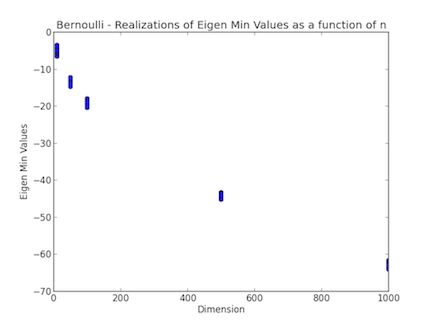
\includegraphics[scale = 0.8]{23bmin.png}}{\caption{:Realization of eigen min values - Symmetric Bernoulli ensemble}\label{4}}
         \ffigbox{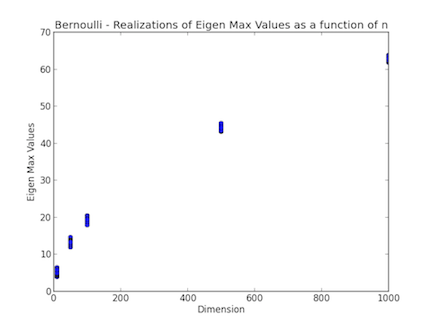
\includegraphics[scale = 0.8]{23bmax.png}}{\caption{:Realization of eigen max values - Symmetric Bernoulli ensemble}\label{25}}
    \end{floatrow}
\end{figure}
\begin{figure}[!htb]
    \begin{floatrow}
         \ffigbox{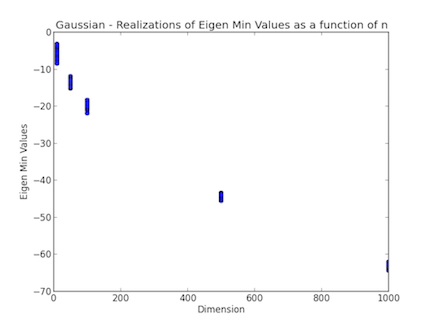
\includegraphics[scale = 0.8]{23gmin.png}}{\caption{:Realization of eigen min values - Gaussian Orthogonal Ensemble}\label{100}}
         \ffigbox{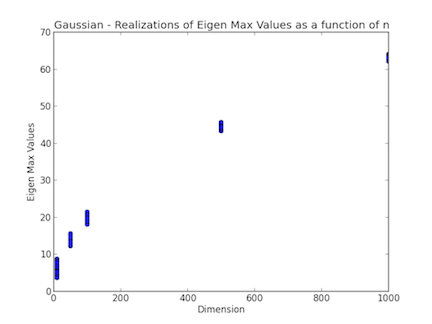
\includegraphics[scale = 0.8]{23gmax.png}}{\caption{:Realization of eigen max values - Gaussian Orthogonal Ensemble}\label{225}}
    \end{floatrow}
\end{figure}
\end{flushleft}
\vspace{20em}
\section*{Ans 24}
\begin{flushleft}
\begin{figure}[!htb]
    \begin{floatrow}
         \ffigbox{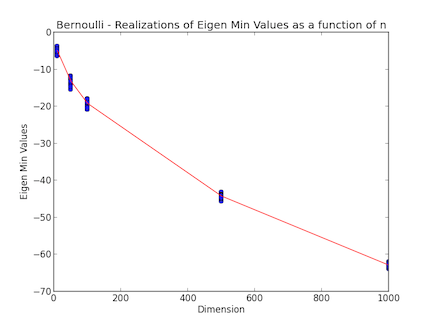
\includegraphics[scale = 0.8]{24bminf.png}}{\caption{:Realization of eigen min values with curve fitting - Symmetric Bernoulli ensemble}\label{4}}
         \ffigbox{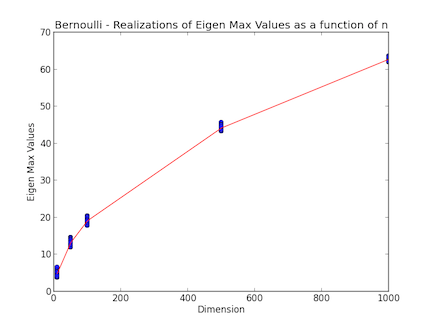
\includegraphics[scale = 0.8]{24bmaxf.png}}{\caption{:Realization of eigen max values with curve fitting - Symmetric Bernoulli ensemble}\label{25}}
    \end{floatrow}
\end{figure}
\begin{figure}[!htb]
    \begin{floatrow}
         \ffigbox{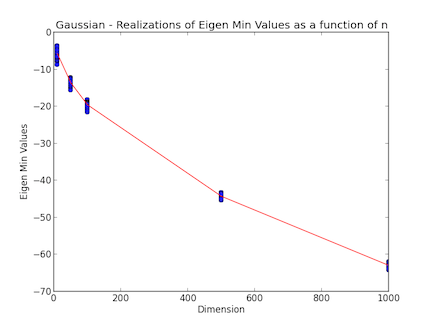
\includegraphics[scale = 0.8]{24gminf.png}}{\caption{:Realization of eigen min values with curve fitting - Gaussian Orthogonal Ensemble}\label{100}}
         \ffigbox{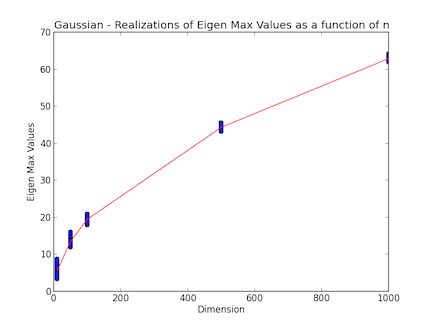
\includegraphics[scale = 0.8]{24gmaxf.png}}{\caption{:Realization of eigen max values with curve fitting - Gaussian Orthogonal Ensemble}\label{225}}
    \end{floatrow}
\end{figure}
\end{flushleft}
\vspace{20em}
\section*{Ans 25}
\begin{flushleft}
\begin{figure}[!htb]
    \begin{floatrow}
         \ffigbox{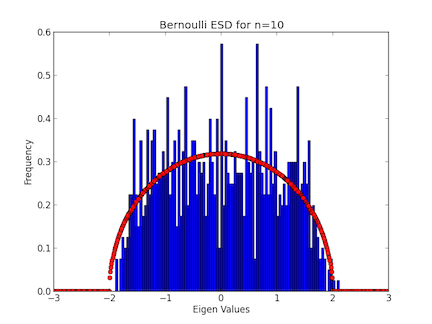
\includegraphics[scale = 0.8]{25_hist_10.png}}{\caption{: Bernoulli - Empirical Spectral Distribution for n = 10}\label{4}}
         \ffigbox{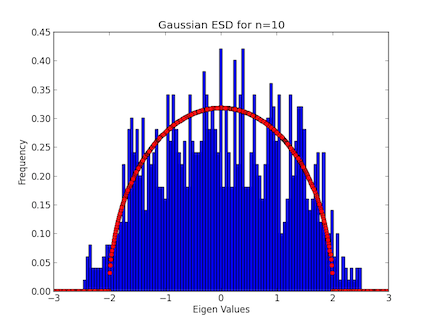
\includegraphics[scale = 0.8]{25_hist_10g.png}}{\caption{:Gaussian - Empirical Spectral Distribution for n = 10}\label{25}}
    \end{floatrow}
\end{figure}
\begin{figure}[!htb]
    \begin{floatrow}
         \ffigbox{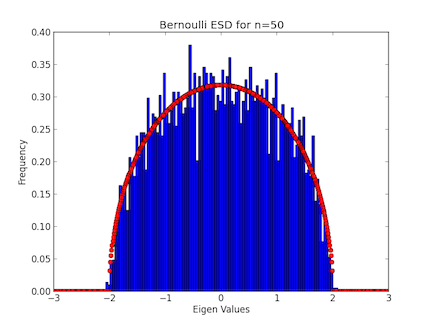
\includegraphics[scale = 0.8]{25_hist_50.png}}{\caption{: Bernoulli - Empirical Spectral Distribution for n = 50}\label{4}}
         \ffigbox{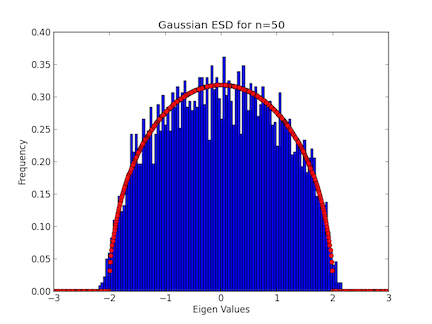
\includegraphics[scale = 0.8]{25_hist_50g.png}}{\caption{:Gaussian - Empirical Spectral Distribution for n = 50}\label{25}}
    \end{floatrow}
\end{figure}
\begin{figure}[!htb]
    \begin{floatrow}
         \ffigbox{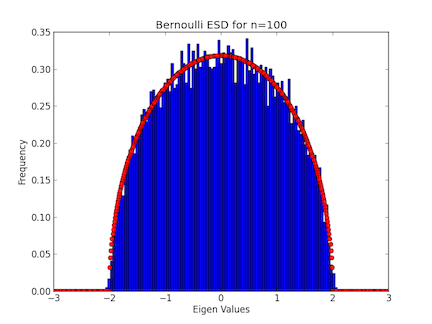
\includegraphics[scale = 0.8]{25_hist_100.png}}{\caption{: Bernoulli - Empirical Spectral Distribution for n = 100}\label{4}}
         \ffigbox{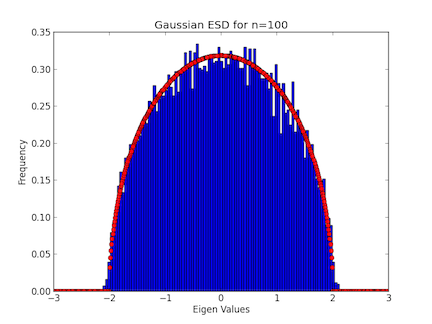
\includegraphics[scale = 0.8]{25_hist_100g.png}}{\caption{:Gaussian - Empirical Spectral Distribution for n = 100}\label{25}}
    \end{floatrow}
\end{figure}
\begin{figure}[!htb]
    \begin{floatrow}
         \ffigbox{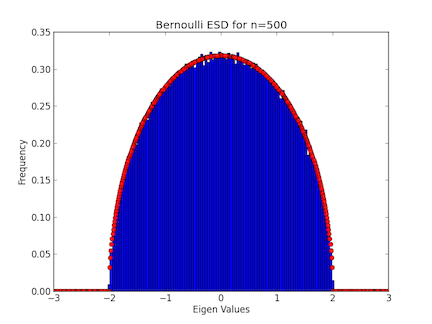
\includegraphics[scale = 0.8]{25_hist_500.png}}{\caption{: Bernoulli - Empirical Spectral Distribution for n = 500}\label{4}}
         \ffigbox{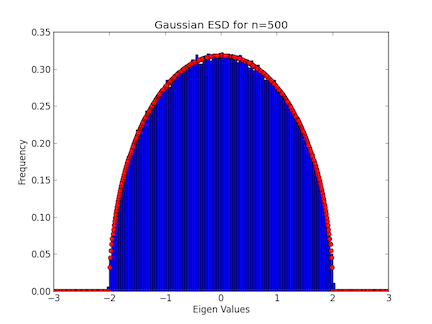
\includegraphics[scale = 0.8]{25_hist_500g.png}}{\caption{:Gaussian - Empirical Spectral Distribution for n = 500}\label{25}}
    \end{floatrow}
\end{figure}
\begin{figure}[!htb]
    \begin{floatrow}
         \ffigbox{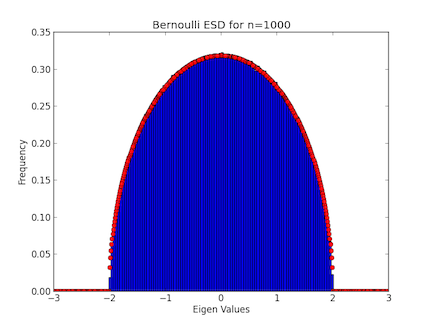
\includegraphics[scale = 0.8]{25_hist_1000.png}}{\caption{: Bernoulli - Empirical Spectral Distribution for n = 1000}\label{4}}
         \ffigbox{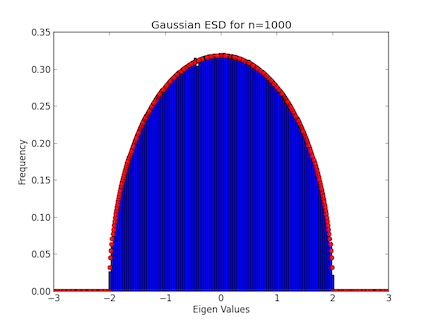
\includegraphics[scale = 0.8]{25_hist_1000g.png}}{\caption{:Gaussian - Empirical Spectral Distribution for n = 1000}\label{25}}
    \end{floatrow}
\end{figure}
\vspace{10em}
We can see that for symmetric matrices with random entries (Bernoulli and Gaussian) the Empirical Spectral Distribution follows the Wigner's Semicircular Law with radius 2 along the x-axis.
\end{flushleft}
\section*{Ans 26}
\begin{flushleft}
\begin{figure}[!htb]
    \begin{floatrow}
         \ffigbox{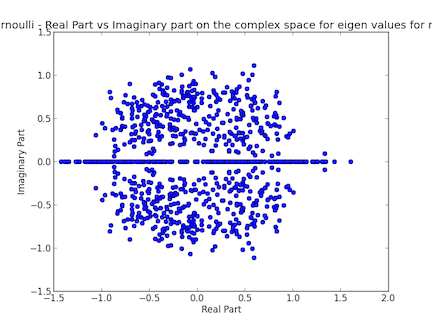
\includegraphics[scale = 0.8]{26_b_10.png}}{\caption{: Bernoulli - Normalized eigenvalues for n = 10}\label{4}}
         \ffigbox{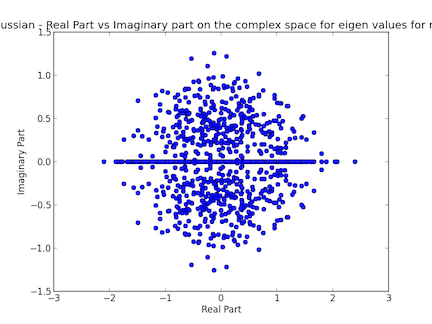
\includegraphics[scale = 0.8]{26_g_10.png}}{\caption{:Gaussian - Normalized eigenvalues for n = 10}\label{25}}
    \end{floatrow}
\end{figure}
\begin{figure}[!htb]
    \begin{floatrow}
         \ffigbox{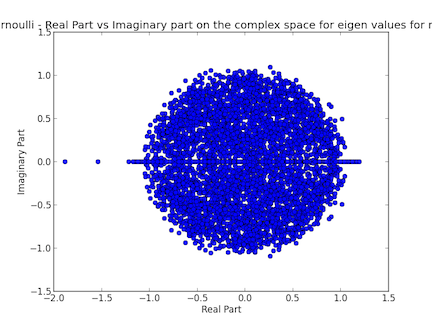
\includegraphics[scale = 0.8]{26_b_50.png}}{\caption{: Bernoulli - Normalized eigenvalues for n = 50}\label{4}}
         \ffigbox{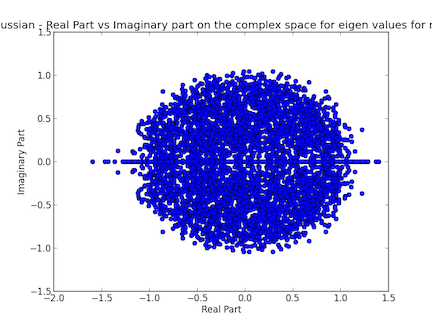
\includegraphics[scale = 0.8]{26_g_50.png}}{\caption{:Gaussian - Normalized eigenvalues for n = 50}\label{25}}
    \end{floatrow}
\end{figure}
\begin{figure}[!htb]
    \begin{floatrow}
         \ffigbox{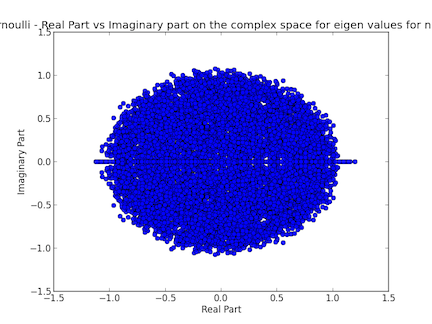
\includegraphics[scale = 0.8]{26_b_100.png}}{\caption{: Bernoulli - Normalized eigenvalues for n = 100}\label{4}}
         \ffigbox{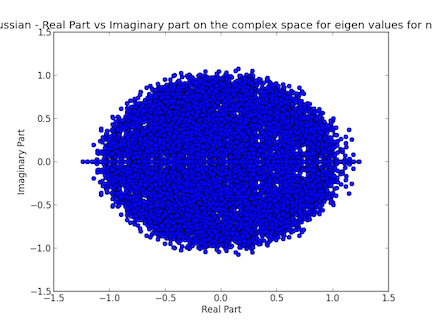
\includegraphics[scale = 0.8]{26_g_100.png}}{\caption{:Gaussian - Normalized eigenvalues for n = 100}\label{25}}
    \end{floatrow}
\end{figure}
\begin{figure}[!htb]
    \begin{floatrow}
         \ffigbox{\includegraphics[scale = 0.8]{26_b_500.png}}{\caption{: Bernoulli - Normalized eigenvalues for n = 500}\label{4}}
         \ffigbox{\includegraphics[scale = 0.8]{26_g_500.png}}{\caption{:Gaussian - Normalized eigenvalues for n = 500}\label{25}}
    \end{floatrow}
\end{figure}
\begin{figure}[!htb]
    \begin{floatrow}
         \ffigbox{\includegraphics[scale = 0.8]{26_b_1000.png}}{\caption{: Bernoulli - Normalized eigenvalues for n = 1000}\label{4}}
         \ffigbox{\includegraphics[scale = 0.8]{26_g_1000.png}}{\caption{:Gaussian - Normalized eigenvalues for n = 1000}\label{25}}
    \end{floatrow}
\end{figure}
\end{flushleft}
\section*{Ans 27}
\begin{flushleft}
The minimum value for the eigenvalues seems to be increasing with dimension and the maximum value of the eigenvalues seems to be decreasing with dimension unlike the symmetric case. 
\end{flushleft}
\end{document}